%!TEX ROOT=../diploma-thesis.tex

\chapter{Přehledové obrázky a sn\'{\i}mky}

\begin{figure}
    \centering
    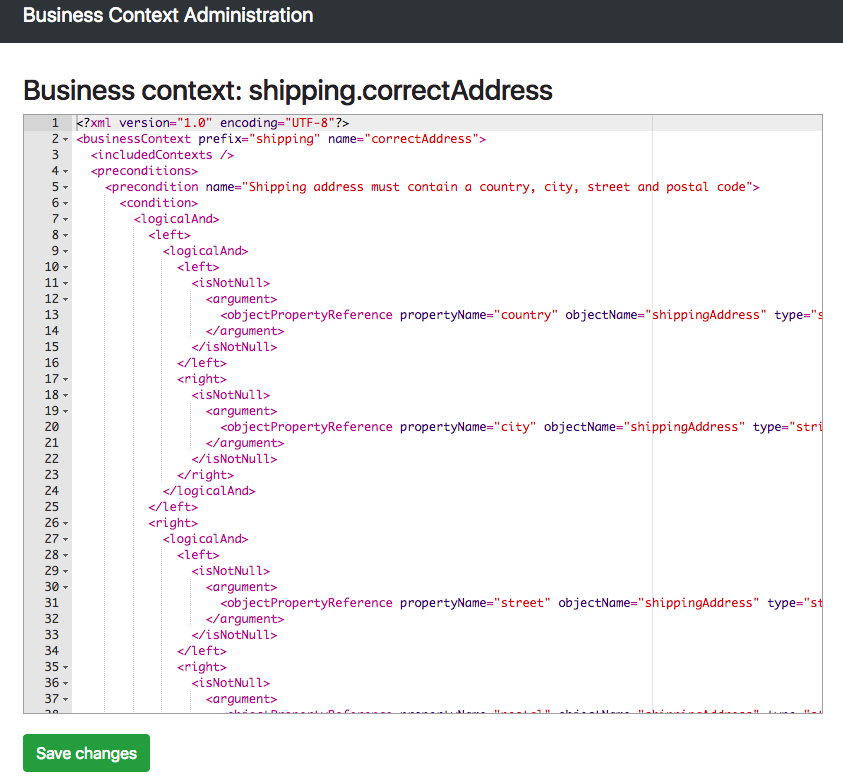
\includegraphics[width=0.9\linewidth]{figures/business-context-edit.png}
    \caption{Formulář pro vytvořen\'{\i} nebo úpravu byznysového kontextu v centráln\'{\i} administraci}
    \label{fig:screenshot-context-edit}
\end{figure}

\begin{figure}
    \centering
    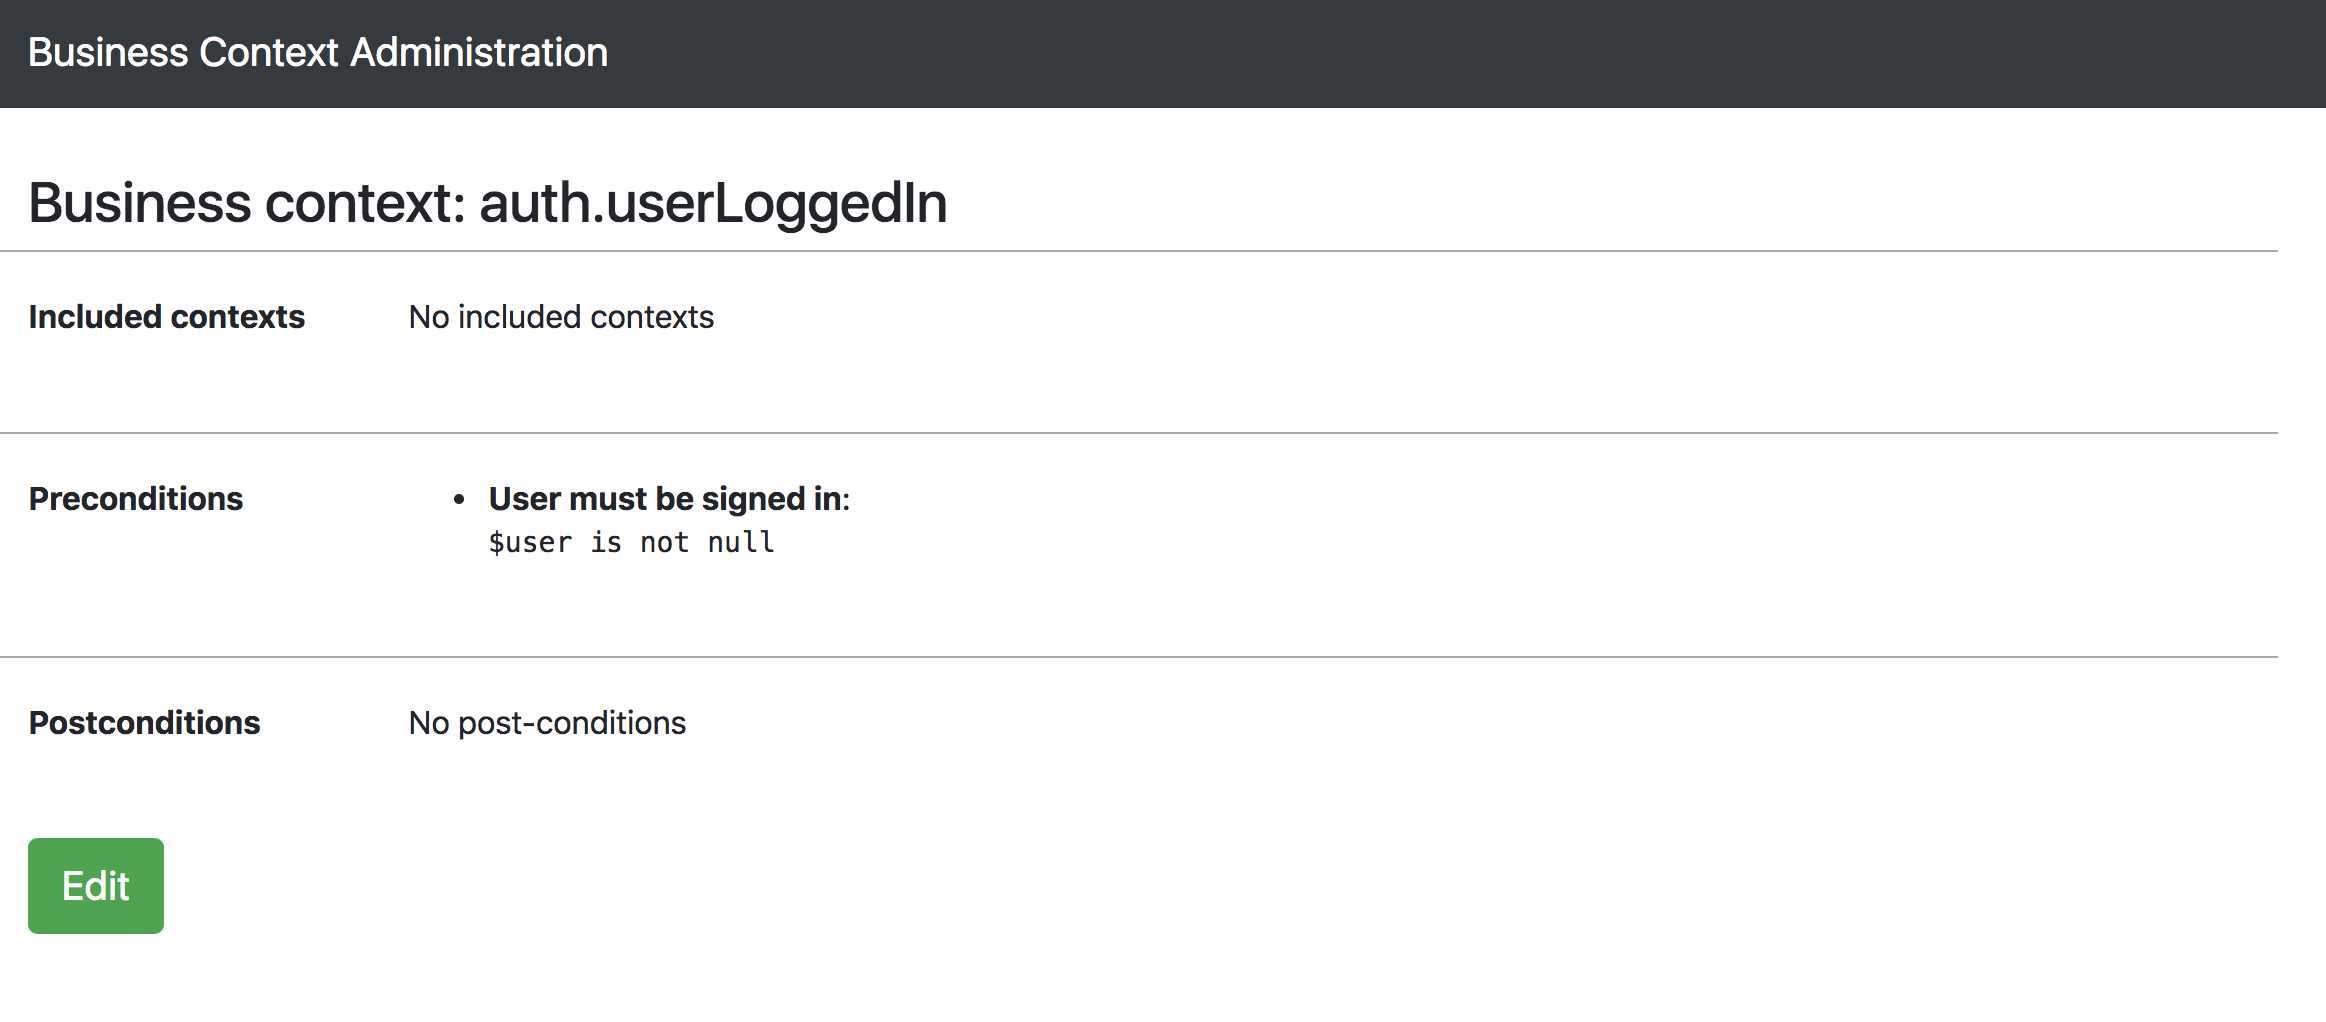
\includegraphics[width=0.9\linewidth]{figures/business-context-detail.png}
    \caption{Detail byznysového kontextu v centráln\'{\i} administraci}
    \label{fig:screenshot-context-detail}
\end{figure}

\begin{sidewaysfigure}[ht]
    \centering
    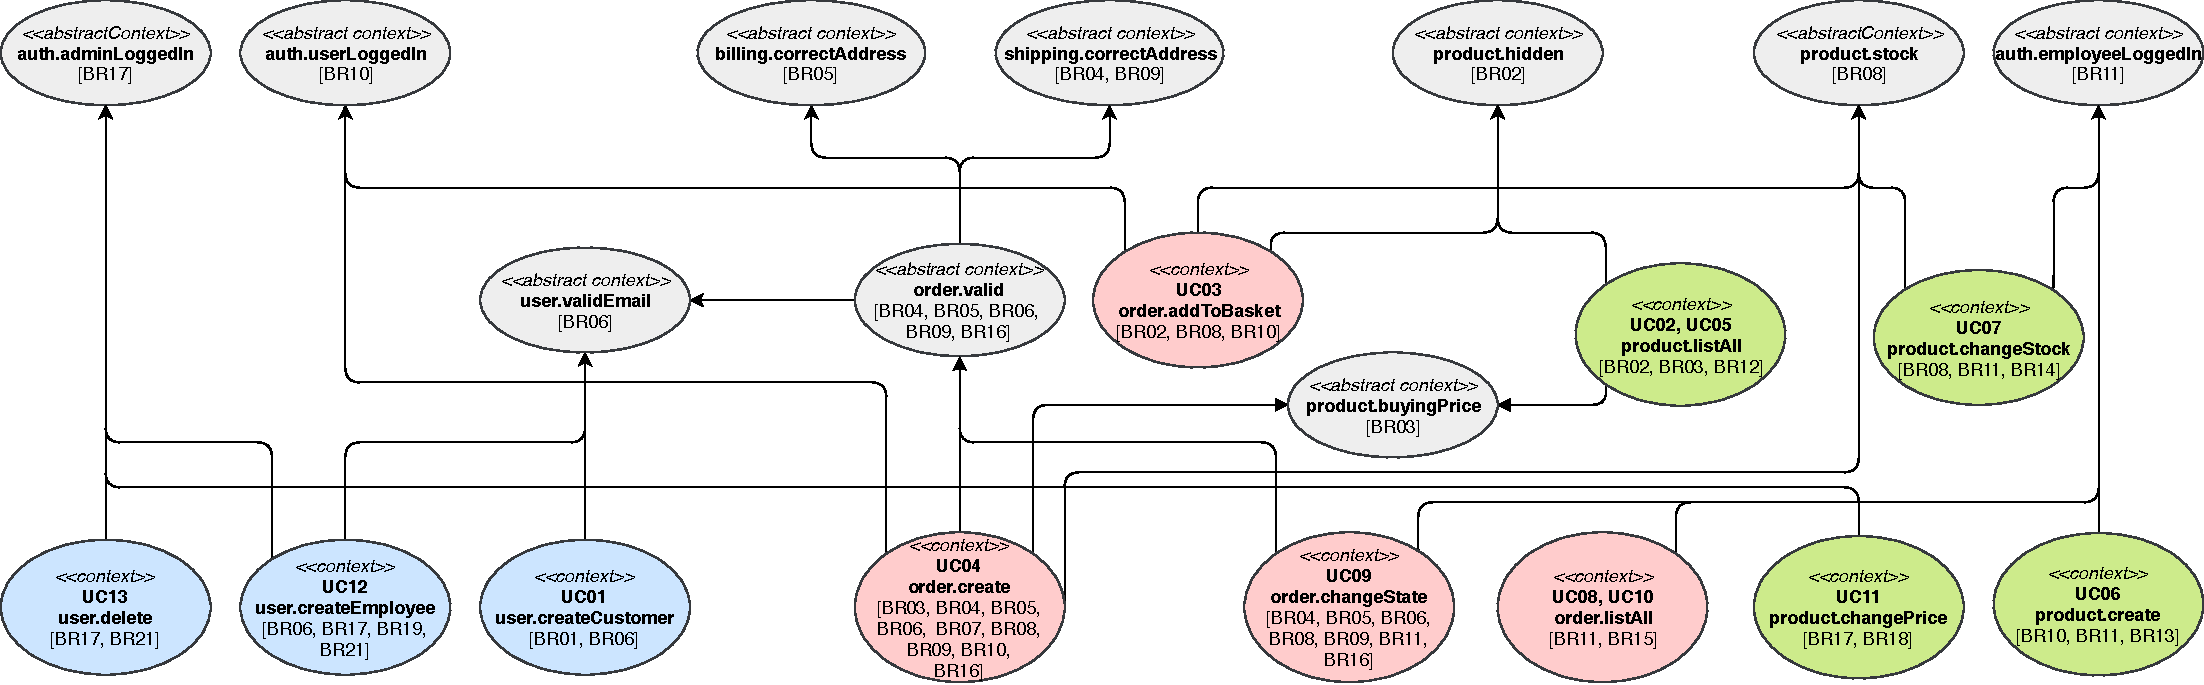
\includegraphics[keepaspectratio=true, width=\linewidth]{figures/example-system-context-hierarchy.pdf}
    \caption{Diagram hirearchie byznysov\'ych kontextů ukázkového systému}
    \label{fig:example-system-context-hirearchy}
\end{sidewaysfigure}

\begin{figure}
    \centering
    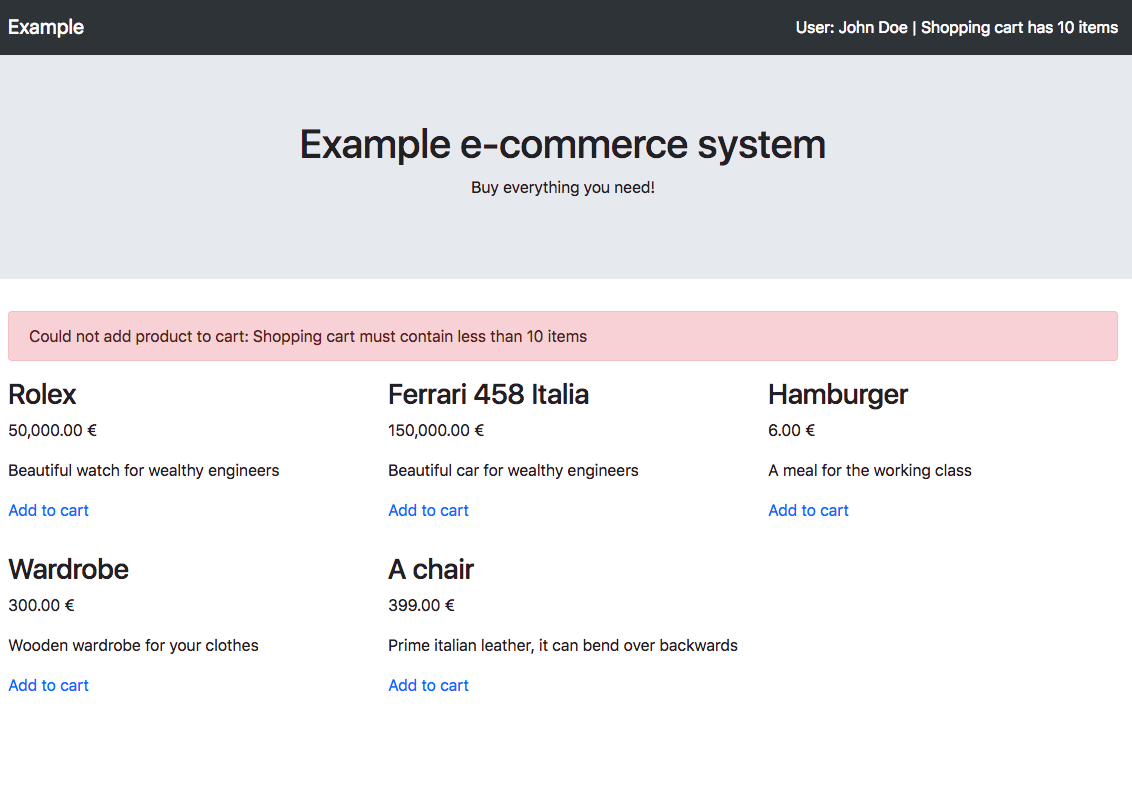
\includegraphics[width=0.9\linewidth]{figures/add-product-to-cart-fail.png}
    \caption{Propagace byznysového pravidla při přidáván\'{\i} produktu do koš\'{\i}ku v ukázkovém systému}
    \label{fig:example-screenshot}
\end{figure}
